% Options for packages loaded elsewhere
\PassOptionsToPackage{unicode}{hyperref}
\PassOptionsToPackage{hyphens}{url}
%
\documentclass[
  11pt,
]{article}
\usepackage{amsmath,amssymb}
\usepackage[]{times}
\usepackage{iftex}
\ifPDFTeX
  \usepackage[T1]{fontenc}
  \usepackage[utf8]{inputenc}
  \usepackage{textcomp} % provide euro and other symbols
\else % if luatex or xetex
  \usepackage{unicode-math}
  \defaultfontfeatures{Scale=MatchLowercase}
  \defaultfontfeatures[\rmfamily]{Ligatures=TeX,Scale=1}
\fi
% Use upquote if available, for straight quotes in verbatim environments
\IfFileExists{upquote.sty}{\usepackage{upquote}}{}
\IfFileExists{microtype.sty}{% use microtype if available
  \usepackage[]{microtype}
  \UseMicrotypeSet[protrusion]{basicmath} % disable protrusion for tt fonts
}{}
\makeatletter
\@ifundefined{KOMAClassName}{% if non-KOMA class
  \IfFileExists{parskip.sty}{%
    \usepackage{parskip}
  }{% else
    \setlength{\parindent}{0pt}
    \setlength{\parskip}{6pt plus 2pt minus 1pt}}
}{% if KOMA class
  \KOMAoptions{parskip=half}}
\makeatother
\usepackage{xcolor}
\IfFileExists{xurl.sty}{\usepackage{xurl}}{} % add URL line breaks if available
\IfFileExists{bookmark.sty}{\usepackage{bookmark}}{\usepackage{hyperref}}
\hypersetup{
  pdftitle={Successor Representations},
  pdfauthor={Julien Vitay},
  hidelinks,
  pdfcreator={LaTeX via pandoc}}
\urlstyle{same} % disable monospaced font for URLs
\usepackage[margin=1in]{geometry}
\usepackage{listings}
\newcommand{\passthrough}[1]{#1}
\lstset{defaultdialect=[5.3]Lua}
\lstset{defaultdialect=[x86masm]Assembler}
\usepackage{graphicx}
\makeatletter
\def\maxwidth{\ifdim\Gin@nat@width>\linewidth\linewidth\else\Gin@nat@width\fi}
\def\maxheight{\ifdim\Gin@nat@height>\textheight\textheight\else\Gin@nat@height\fi}
\makeatother
% Scale images if necessary, so that they will not overflow the page
% margins by default, and it is still possible to overwrite the defaults
% using explicit options in \includegraphics[width, height, ...]{}
\setkeys{Gin}{width=\maxwidth,height=\maxheight,keepaspectratio}
% Set default figure placement to htbp
\makeatletter
\def\fps@figure{htbp}
\makeatother
\setlength{\emergencystretch}{3em} % prevent overfull lines
\providecommand{\tightlist}{%
  \setlength{\itemsep}{0pt}\setlength{\parskip}{0pt}}
\setcounter{secnumdepth}{5}
\newlength{\cslhangindent}
\setlength{\cslhangindent}{1.5em}
\newlength{\csllabelwidth}
\setlength{\csllabelwidth}{3em}
\newlength{\cslentryspacingunit} % times entry-spacing
\setlength{\cslentryspacingunit}{\parskip}
\newenvironment{CSLReferences}[2] % #1 hanging-ident, #2 entry spacing
 {% don't indent paragraphs
  \setlength{\parindent}{0pt}
  % turn on hanging indent if param 1 is 1
  \ifodd #1
  \let\oldpar\par
  \def\par{\hangindent=\cslhangindent\oldpar}
  \fi
  % set entry spacing
  \setlength{\parskip}{#2\cslentryspacingunit}
 }%
 {}
\usepackage{calc}
\newcommand{\CSLBlock}[1]{#1\hfill\break}
\newcommand{\CSLLeftMargin}[1]{\parbox[t]{\csllabelwidth}{#1}}
\newcommand{\CSLRightInline}[1]{\parbox[t]{\linewidth - \csllabelwidth}{#1}\break}
\newcommand{\CSLIndent}[1]{\hspace{\cslhangindent}#1}
\usepackage{setspace}
\onehalfspacing
\usepackage{titling}
\pretitle{\begin{center}\begin{bfseries}\begin{huge}}
\posttitle{\end{huge}\end{bfseries}\end{center}}
\renewcommand{\linethickness}{0.4pt}
\usepackage{xcolor}
\usepackage[colorlinks=true]{hyperref}
\definecolor{commentsColor}{rgb}{0.197495, 0.197587, 0.197464}
\definecolor{keywordsColor}{rgb}{0.000000, 0.000000, 0.635294}
\definecolor{stringColor}{rgb}{0.558215, 0.000000, 0.135316}
\lstset{backgroundcolor=\color{white}, basicstyle=\footnotesize\ttfamily, breakatwhitespace=false, breaklines=true, captionpos=none, keepspaces=true, keywordstyle=\color{keywordsColor}\bfseries, language=Python, tabsize=4}
\ifLuaTeX
  \usepackage{selnolig}  % disable illegal ligatures
\fi

\title{Successor Representations}
\usepackage{etoolbox}
\makeatletter
\providecommand{\subtitle}[1]{% add subtitle to \maketitle
  \apptocmd{\@title}{\par {\large #1 \par}}{}{}
}
\makeatother
\subtitle{An introduction}
\author{Julien Vitay}
\date{}

\begin{document}
\maketitle

{
\setcounter{tocdepth}{3}
\tableofcontents
}
\begin{lstlisting}[language=Python]
from ANNarchy import *

setup(dt=1.0)

pop = Population(1000, Izhikevich)

compile()
\end{lstlisting}

\hypertarget{motivation}{%
\section{Motivation}\label{motivation}}

\hypertarget{model-free-vs.-model-based-rl}{%
\subsection{Model-free vs.~model-based
RL}\label{model-free-vs.-model-based-rl}}

There are two main families of \textbf{reinforcement learning} (RL)
(\protect\hyperlink{ref-Sutton2017}{Sutton and Barto, 2017}) algorithms:

\begin{itemize}
\tightlist
\item
  \textbf{Model-free} (MF) methods estimate the value of a state
  \(V^\pi(s)\) or of a state-action pair \(Q^\pi(s, a)\) by sampling
  trajectories and averaging the obtained returns (Monte-Carlo control),
  or by estimating the Bellman equations (Temporal difference - TD):
\end{itemize}

\[V^\pi(s) = \mathbb{E}_{\pi} [\sum_{k=0} \gamma^k \, r_{t+k+1}  | s_t = s] = \mathbb{E}_{\pi} [r_{t+1} + \gamma \, V^\pi(s_{t+1})  | s_t = s]\]

\[Q^\pi(s, a) = \mathbb{E}_{\pi} [\sum_{k=0} \gamma^k \, r_{t+k+1}  | s_t = s, a_t = a] = \mathbb{E}_{\pi} [r_{t+1} + \gamma \, Q^\pi(s_{t+1}, a_{t+1})  | s_t = s, a_t = a]\]

\begin{itemize}
\tightlist
\item
  \textbf{Model-based} (MB) methods use (or learn) a model of the
  environment - transition probabilities \(p(s\_{t+1} | s\_t, a\_t)\)
  and reward probabilities \(r(s\_t, a\_t, s\_{t+1})\) - and use it to
  plan trajectories maximizing the theoretical return, either through
  some form of forward planning (search tree) or using dynamic
  programming (solving the Bellman equations directly).
\end{itemize}

\[\pi^* = \text{argmax}_{\pi} \; p(s_0) \, \sum_{t=0}^\infty \gamma^t \, p(s_{t+1} | s_t, a_t) \, \pi(s_t, a_t) \, r(s_t, a_t, s_{t+1})\]

\[V^*(s) = \max_a \sum_{s'} p(s' | s, a) \, (r(s_t, a, s')+ \gamma \, V^*(s'))\]

The main advantage of model-free methods is their speed: they
\emph{cache} the future of the system into value functions. When having
to take a decision at time \(t\), we only need to look at the action
with the highest Q-value in the state \(s\_t\) and take it. If the
Q-values are optimal, this is the optimal policy. Oppositely,
model-based algorithms have to plan sequentially in the state-action
space, which can be very long if the problem has a long temporal
horizon.

The main drawback of MF methods is their \emph{inflexibility} when the
reward distribution changes. When the reward associated with a
transition changes (the source of reward has vanished, its nature has
changed, the rules of the game have changed, etc), each action leading
to that transition has to be experienced multiple times before the
corresponding values reflect that change. This is due to the use of the
\textbf{temporal difference} (TD) algorithm, where the \textbf{reward
prediction error} (RPE) is used to update values:

\[\delta_t = r_{t+1} + \gamma \, V^\pi(s_{t+1}) - V^\pi(s_t)\]

\[\Delta V^\pi(s_t) = \alpha \, \delta_t\]

When the reward associated to a transition changes drastically, only the
last state (or action) is updated after that experience (unless we use
eligibility traces). Only multiple repetitions of the same trajectory
would allow changing the initial decisions. This is opposite to MB
methods, where a change in the reward distribution would very quickly
influence the planning of the optimal trajectory. In MB, the reward
probabilities can be estimated with:

\[
    \Delta r(s_t, a_t, s_{t+1}) = \alpha \, (r_{t+1} - r(s_t, a_t, s_{t+1}))
\]

with \(r_{t+1}\) being the reward obtained during one sampled
transition. The transition probabilities can also be learned from
experience using:

\[
    \Delta p(s' | s_t, a_t) = \alpha \, (\mathbb{I}(s_{t+1} = s') - p(s' | s_t, a_t))
\]

where \(\mathbb{I}(b)\) is 1 when \(b\) is true, 0 otherwise. Depending
on the learning rate, changes in the environment dynamics can be very
quickly learned by MB methods, as updates do not depend on other
estimates (there is no bootstrapping contrary to TD).

\hypertarget{goal-directed-behavior-vs.-habits}{%
\subsection{Goal-directed behavior
vs.~habits}\label{goal-directed-behavior-vs.-habits}}

The model-free RPE has become a very influential model of dopaminergic
(DA) activation in the ventral tegmental area (VTA) and substantia nigra
pars compacta (SNc). At the beginning of classical Pavlovian
conditioning, DA cells react phasically to unconditioned stimuli (US,
rewards). After enough conditioning trials, DA cells only react to
conditioned stimuli (CS), i.e.~stimuli which predict the delivery of a
reward. Moreover, if the reward is omitted, DA cells exhibit a pause in
firing. This pattern of activation corresponds to the RPE: DA cells
respond to unexpected reward events, either positively when more reward
than expected is received, or negatively when less reward is delivered.
The simplicity of this model has made RPE a successful model of DA
activity (but see Vitay and Hamker
(\protect\hyperlink{ref-Vitay2014}{2014}) for a more detailed model).

A similar but not identical functional dichotomy as MF/MB opposes
deliberative \textbf{goal-directed} behavior and inflexible
stimulus-response associations called \textbf{habits}
(\protect\hyperlink{ref-Dickinson2002}{Dickinson and Balleine, 2002}).
Goal-directed behavior is sensitive to reward devaluation: if an outcome
was previously rewarding but ceases to be (for example, a poisonous
product is injected into some food reward, even outside the conditioning
phase), goal-directed behavior would quickly learn to avoid that
outcome, while habitual behavior will continue to seek for it.
Over-training can transform goal-directed behavior into habits
(\protect\hyperlink{ref-Corbit2011}{Corbit and Balleine, 2011}). Habits
are usually considered as a model-free learning behavior, while
goal-directed behavior implies the use of a world model. The \emph{dual
system theory} discusses the arbitration mechanisms necessary to
coordinate these two learning frameworks
(\protect\hyperlink{ref-Lee2014}{Lee et al., 2014}).

Both forms of behavior are thought to happen concurrently in the brain,
with model-based / goal-directed behavior classically assigned to the
prefrontal cortex and the hippocampus and model-free / habitual behavior
mapped to the ventral basal ganglia and the dopaminergic system.
However, recent results and theories suggest that these two functional
systems are largely overlapping and that even dopamine firing might
reflect model-based processes (\protect\hyperlink{ref-Doll2012}{Doll et
al., 2012}; \protect\hyperlink{ref-Miller2018}{Miller et al., 2018}). It
is yet to be understood how these two extreme mechanisms of the RL
spectrum might coexist in the brain and be coordinated: successor
representations might provide us with additional useful insights into
the functioning of the brain.

\hypertarget{successor-representations-in-reinforcement-learning}{%
\section{Successor representations in reinforcement
learning}\label{successor-representations-in-reinforcement-learning}}

\hypertarget{main-idea}{%
\subsection{Main idea}\label{main-idea}}

The original formulation of \textbf{successor representations} (SR) is
actually not recent (\protect\hyperlink{ref-Dayan1993}{Dayan, 1993}),
but it is subject to a revival since a couple of years with the work of
Samuel J. Gershman, e.g. (\protect\hyperlink{ref-Gardner2018}{Gardner et
al., 2018}; \protect\hyperlink{ref-Gershman2012}{Gershman et al., 2012};
\protect\hyperlink{ref-Gershman2018}{Gershman, 2018};
\protect\hyperlink{ref-Momennejad2017a}{Momennejad et al., 2017};
\protect\hyperlink{ref-Stachenfeld2017}{Stachenfeld et al., 2017}).

The SR algorithm learns two quantities:

\begin{enumerate}
\def\labelenumi{\arabic{enumi}.}
\tightlist
\item
  The expected immediate reward received after each state:
\end{enumerate}

\[
    r(s) = \mathbb{E}_{\pi} [r_{t+1} | s_t = s]
\]

\begin{enumerate}
\def\labelenumi{\arabic{enumi}.}
\setcounter{enumi}{1}
\tightlist
\item
  The expected discounted future state occupancy (the \textbf{SR}
  itself):
\end{enumerate}

\[
    M(s, s') = \mathbb{E}_{\pi} [\sum_{k=0}^\infty \gamma^k \, \mathbb{I}(s_{t+k+1} = s') | s_t = s]
\]

I omit here the dependency of \(r\) and \(M\) on the policy itself in
the notation, but it is of course implicitly there.

The SR represents the fact that a state \(s'\) can be reached after
\(s\), with a value decreasing with the temporal gap between the two
states: states occurring in rapid succession will have a high SR, very
distant states will have a low SR. If \(s'\) happens consistently before
\(s\), the SR should be 0 (causality principle). This is in principle
similar to model-based RL, but without an explicit representation of the
transition structure: it only represents how states are temporally
correlated, not which action leads to which state.

The value of a state \(s\) is then defined by:

\[
    V^\pi(s) = \sum_{s'} M(s, s') \, r(s')
\]

The value of a state \(s\) depends on which states \(s'\) can be visited
after it (following the current policy, implicitly), how far in the
future they will happen (discount factor in \(M(s, s')\)) and how much
reward can be obtained immediately in those states (\(r(s')\)). Note
that it is merely a rewriting of the definition of the value of a state,
with rewards explicitly separated from state visitation and time
replaced by succession probabilities:

\[V^\pi(s_t) = \mathbb{E}_{\pi} [\sum_{k=0} \gamma^k \, r_{t+k+1}] = \mathbb{E}_{\pi} [\sum_{k=0} r(s_{t+k+1}) \times (\gamma^k \, \mathbb{I}(s_{t+k+1}))]\]

The SR also obeys a recursive relationship similar to the Bellman
equation, as it is based on a discounted sum:

\[
    M(s_t, s') = \mathbb{I}(s_t = s') + \gamma \, M(s_{t+1}, s')
\]

The discounted probability of arriving in \(s'\) after being in \(s\_t\)
is one if we are already in \(s'\), and gamma times the discounted
probability of arriving in \(s'\) after being in the next state
\(s\_{t+1}\) otherwise.

This recursive relationship implies that we are going to be able to
estimate the SR \(M(s, s')\) using a \textbf{sensory prediction error}
(SPE) similar to the TD RPE
(\protect\hyperlink{ref-Gershman2012}{Gershman et al., 2012}):

\[
    \delta^\text{SR}_t = \mathbb{I}(s_t = s') + \gamma \, M(s_{t+1}, s') - M(s_t, s')
\]

\[
    \Delta M(s_t, s') = \alpha \, \delta^\text{SR}_t
\]

The SPE states that the expected occupancy for states that are visited
more frequently than expected (positive sensory prediction error) should
be increased, while the expected occupancy for states that are visited
less frequently than expected (negative sensory prediction error) should
be decreased. In short: is arriving in this new state surprising? It
should be noted that the SPE is defined over all possible successor
states \(s'\), so the SPE is actually a vector.

We can already observe that SR is a trade-off between MF and MB methods.
A change in the reward distribution can be quickly tracked by SR
algorithms, as the immediate reward \(r(s)\) can be updated with:

\[
    \Delta r(s) = \alpha \, (r_{t+1} - r(s))
\]

However, the SR \(M(s, s')\) uses other estimates for its update
(bootstrapping), so changes in the transition structure may take more
time to propagate to all state-state discounted occupancies
(\protect\hyperlink{ref-Gershman2018}{Gershman, 2018}).

\hypertarget{linear-function-approximation}{%
\subsection{Linear function
approximation}\label{linear-function-approximation}}

Before looking at the biological plausibility of this algorithm, we need
to deal with the \textbf{curse of dimensionality}. The SR \(M(s, s')\)
is a matrix associating each state of the system to all other states
(size \(|\mathcal{S}| \times |\mathcal{S}|\)). This is of course
impracticable for most problems and we need to rely on function
approximation. The simplest solution is to represent each state \(s\) by
a set of \(d\) features \([f\_i(s)]\_{i=1}^d\). Each feature can for
example be the presence of an object in the scene, some encoding of the
position of the agent in the world, etc. The SR for a state \(s\) only
needs to predict the expected discounted probability that a feature
\(f_j\) will be observed in the future, not the complete state
representation. This should ensure generalization across states, as only
the presence of relevant features is needed. The SR can be linearly
approximated by:

\[
    M_j(s) = \sum_{i=1}^d w_{i, j} \, f_i(s)
\]

The expected discounted probability of observing the feature \(f\_j\) in
the future is defined as a weighted sum of the features of the state
\(s\). The value of a state is now defined as:

\[
    V^\pi(s) = \sum_{j=1}^d M_j(s) \, r(f_j) = \sum_{j=1}^d r(f_j) \, \sum_{i=1}^d w_{i, j} \, f_i(s)
\]

where \(r(f\_j)\) is the expected immediate reward when observing the
feature \(f\_j\), what can be easily tracked as before. Computing the
value of a state based on the SR now involves a double sum over a
\(d \times d\) matrix, \(d\) being the number of features, what should
generally be much more tractable than over the total number of states
squared.

As we use linear approximation, the learning rule for the weights
\(w\_{i, j}\) becomes linearly dependent on the SPE:

\[
    \delta^\text{SR}_t(f_j) = f_j(s_t) + \gamma \, M_j(s_{t+1}) - M_j(s)
\]

\[
    \Delta w_{i, j} = \alpha \, \delta^\text{SR}_t(f_j) \, f_i(s_t)
\]

The SPE tells us how surprising is each feature \(f\_j\) when being in
the state \(s_t\). This explains the term \emph{sensory prediction
error}: we are now not learning based on how surprising rewards are
anymore, but on how surprising the sensory features of the outcome are.
Did I expect that door to open at some point? Should this event happen
soon? What kind of outcome is likely to happen? As the SPE is now a
vector for all sensory features, we see why successor representation
have a great potential: instead of a single scalar RPE dealing only with
reward magnitudes, we now can learn from very diverse representations
describing the various relevant dimensions of the task. It can then deal
with different rewards: food and monetary rewards are treated the same
by RPEs, while we can distinguish them with SPEs.

The main potential problem is of course to extract the relevant features
for the task, either by hand-engineering them or through learning (one
could work in the latent space of a variational autoencoder, for
example). Feature-based state representations still have to be Markovian
for SR to work. It is also possible to use non-linear function
approximators such as deep networks
(\protect\hyperlink{ref-Barreto2016}{Barreto et al., 2016};
\protect\hyperlink{ref-Kulkarni2016}{Kulkarni et al., 2016};
\protect\hyperlink{ref-Ma2018}{Ma et al., 2018};
\protect\hyperlink{ref-Machado2018}{Machado et al., 2018};
\protect\hyperlink{ref-Zhang2016}{Zhang et al., 2016}), but this is out
of the scope of this post.

\hypertarget{successor-representations-of-actions}{%
\subsection{Successor representations of
actions}\label{successor-representations-of-actions}}

The previous sections focused on the successor representation of states
to obtain the value function \(V^\pi(s)\). The same idea can be applied
to state-action pairs and their \(Q^\pi(s, a)\) values. The Q-value of a
state action pair can be defined as:

\[
    Q^\pi(s, a) = \sum_{s', a'} M(s, a, s', a') \, r(s', a')
\]

where \(r(s', a')\) is the expected immediate reward obtained after
\((s', a')\) and \(M(s, a, s', a')\) is the SR between the pairs
\((s, a)\) and \((s', a')\) as in (Momennejad et al., 2017). Ducarouge
and Sigaud (2017) use a SR representation between a state-action pair
\((s, a)\) and a successor state \(s'\):

\[
    Q^\pi(s, a) = \sum_{s'} M(s, a, s') \, r(s')
\]

In both cases, the SR can be learned using a sensory prediction error,
such as:

\[
    \delta^\text{SR}_{s_t, a_t} = \mathbb{I}(s_t = s') + \gamma \, M(s_{t+1}, a_{t+1}, s') - M(s_t, a_t, s')
\]

Note that eligibility traces can be used in SR learning as easily as in
TD methods.

\hypertarget{successor-representations-in-neuroscience}{%
\section{Successor representations in
neuroscience}\label{successor-representations-in-neuroscience}}

\hypertarget{human-goal-directed-behavior}{%
\subsection{Human goal-directed
behavior}\label{human-goal-directed-behavior}}

So great, we now have a third form of reinforcement learning. Could it
be the missing theory to explain human reinforcement learning and the
dichotomy goal-directed behavior / habits?

Momennejad et al.~(2017) designed a two-steps sequential learning task
with reward and transition revaluations. In the first learning phase,
the subjects are presented with sequences of images (the states) and
obtain different rewards (Fig. 1). The sequence
\(1 \rightarrow 3 \rightarrow 5\) is rewarded with 10 dollars while the
sequence \(2 \rightarrow 4 \rightarrow 6\) is rewarded with 1 dollar
only. Successful learning is tested by asking the participant whether
he/she prefers the states 1 or 2 (the answer is obviously 1).

\begin{figure}
\centering
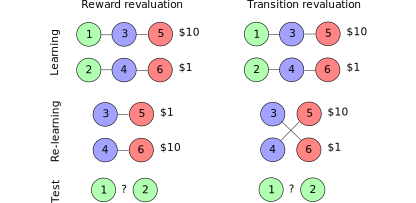
\includegraphics[width=0.6\textwidth,height=\textheight]{img/sr_momennejad.svg}
\caption{\textbf{Figure 1.} Two-steps sequential learning task of
Momennejad et al.~(2017).}
\end{figure}

In the reward revaluation task, the transitions \(3 \rightarrow 5\) and
\(4 \rightarrow 6\) are experienced again in the re-learning phase, but
this time with reversed rewards (1 and 10 dollars respectively). In the
transition revaluation task, the transitions \(3 \rightarrow 6\) and
\(4 \rightarrow 5\) are now experienced, but the states \(5\) and \(6\)
still receive the same amount of reward. The preference for \(1\) or
\(2\) is again tested at the end of the re-learning phase (\(2\) should
now be preferred in both tasks) and a revaluation score is computed (how
much the subject changes his preference between the two phases).

What would the different ML methods predict?

\begin{itemize}
\item
  Model-free methods would not change their preference in both
  conditions. The value of the \(3 \rightarrow 5\) and
  \(4 \rightarrow 6\) transitions (reward revaluation) or
  \(3 \rightarrow 6\) and \(4 \rightarrow 5\) (transition revaluation)
  would change during the re-learning phase, but the transitions
  \(1 \rightarrow 3\) and \(2 \rightarrow 4\) are never experienced
  again, so the value of the states \(1\) and \(2\) can only stay the
  same, even with eligibility traces.
\item
  Model-based methods would change their preference in both conditions.
  The reward and transition probabilities would both be re-learned
  completely to reflect the change, so the new value of \(1\) and \(2\)
  can be computed correctly using dynamic programming.
\item
  Successor representation methods would adapt to the reward revaluation
  (\(r(s)\) will quickly fit the new reward distribution for the states
  \(5\) and \(6\)), but not to the transition revaluation: \(6\) is
  never a successor state of \(1\) in the re-learning phase, so the SR
  matrix will not be updated for the states \(1\) and \(2\).
\end{itemize}

We have three different mechanisms with testable predictions on these
two tasks: the human experiments should tell us which method is the best
model of human RL. Well\ldots{} Not really.

\begin{figure}
\centering
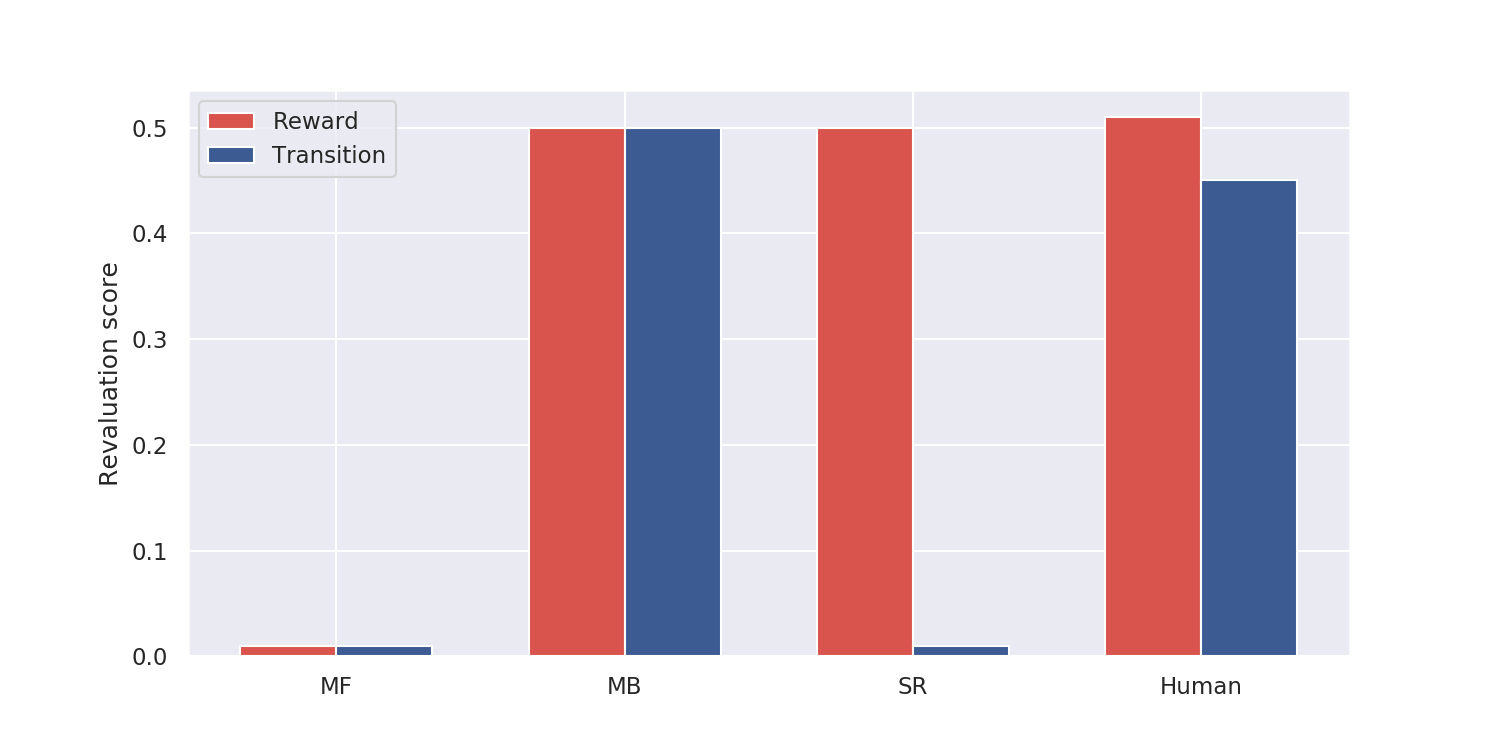
\includegraphics{img/sr_results.png}
\caption{\textbf{Figure 2.} Revaluation score in the reward (red) and
transition (blue) revaluation conditions for the model-free (MF),
model-based (MB), successor representation (SR) and human data as
reported in Momennejad et al.~(2017).}
\end{figure}

Human participants show a revaluation behavior in the two conditions
(reward and transition) somehow in between the model-based and successor
representation algorithms. The difference between the reward and
transition conditions is statistically significant, so unlike MB, but
not as dramatic as for SR. The authors propose a hybrid SR-MB model,
linearly combining the outputs of the MB and SR algorithms, and fit it
to the human data to obtain a satisfying match. A second task requiring
the model to actually take actions confirms this observation.

It is hard to conclude anything definitive from this model and the
somehow artificial fit to the data. Reward revaluation was the typical
test to distinguish between MB and MF processes, or between
goal-directed behavior and habits. This paper suggests that transition
revaluation (and policy revaluation, investigated in the second
experiment) might allow distinguishing between MB and SR mechanisms,
supporting the existence of SR mechanisms in the brain. How MB and SR
might interact in the brain and whether there is an arbitration
mechanism between the two is still an open issue. (Russek et al., 2017)
has a very interesting discussion on the link between MF and MB
processes in the brain, based on different versions of the SR.

\hypertarget{neural-substrates-of-successor-representations}{%
\subsection{Neural substrates of successor
representations}\label{neural-substrates-of-successor-representations}}

In addition to describing human behavior at the functional level, the SR
might also allow to better understand the computations made by the areas
involved in goal-directed behavior, in particular the prefrontal cortex,
the basal ganglia, the dopaminergic system, and the hippocampus. The key
idea of Gershman and colleagues is that the SR \(M(s, s')\) might be
encoded in the place cells of the hippocampus (Stachenfeld et al.,
2017), which are known to be critical for reward-based navigation. The
sensory prediction error (SPE \(\delta^\text{SR}\_t\)) might be encoded
in the activation of the dopaminergic cells in VTA (or in a
fronto-striatal network), driving learning of the SR in the hippocampus
(Gardner et al., 2018), while the value of a state
\(V^\pi(s) = \sum_{s'} M(s, s') \, r(s')\) could be computed either in
the prefrontal cortex (ventromedial or orbitofrontal) or in the ventral
striatum (nucleus accumbens in rats), ultimately allowing action
selection in the dorsal BG.

\hypertarget{dopamine-as-a-spe}{%
\subsubsection{Dopamine as a SPE}\label{dopamine-as-a-spe}}

The most striking prediction of the SR hypothesis is that the SPE is a
vector of prediction errors, with one element per state (in the original
formulation) or per reward feature (using linear function approximation,
section 2.2). This contrasts with the classical RPE formulation, where
dopaminergic activation is a single scalar signal driving reinforcement
learning in the BG and prefrontal cortex. Although this would certainly
be an advantage in terms of functionality and flexible learning, it
remains to be shown whether VTA actually encodes such a feature-specific
signal.

Neurons in VTA have a rather uniform response to rewards or
reward-predicting cues, encoding mostly the value of the outcome
regardless its sensory features, except for those projecting to the tail
of the striatum which mostly respond to threats and punishments
(Watabe-Uchida and Uchida, 2019). The current state of knowledge seems
to rule out VTA as a direct source of SPE signals.

Interestingly, Oemisch et al.~(2019) showed that feature-specific
prediction errors signals (analogous to the SPE with linear
approximation) are detected in the fronto-striatal network including the
anterior cingulate area (ACC), dorsolateral prefrontal cortex (dlPFC),
dorsal striatum and ventral striatum (VS) / nucleus accumbens (NAcc).
These SPE-like signals appear shortly after non-specific RPE signals,
first in ACC and then in the rest of the network. This suggests that SPE
would actually be the result of a more complex calculation than proposed
in the SR hypothesis, involving a network of interconnected areas. A
detailed neuro-computational model of this network still has to be
proposed.

\hypertarget{hippocampus-as-a-predictive-map}{%
\subsubsection{Hippocampus as a predictive
map}\label{hippocampus-as-a-predictive-map}}

Another interesting prediction of the SR hypothesis is that the
hippocampus might be the site where the SR matrix is represented
(Stachenfeld et al., 2017). In navigation tasks, the so-called
\textbf{place cells} in the hippocampus exhibit roughly circular
receptive fields centered on different locations in the environment
(O'Keefe and Nadel, 1978). Altogether, place cells are thought to
provide a sparse code of the animal's location. Strikingly, place fields
change with the environment: moving the animal from a circular to a
rectangular environment, or introducing barriers, modifies the
distribution of place fields. Additionally, \textbf{grid cells} in the
entorhinal cortex (reciprocally connected to the hippocampus) show a
hexagonal grid pattern of receptive fields, i.e.~a single grid cell
responds for several positions of the animal inside the environment
(Hafting et al., 2005). Grid cells' receptive fields also depend on the
environment and have been shown to depend on place cells, not the other
way around. The mechanism behind the flexibility of place and grid
fields is still to be understood.

Stachenfeld et al.~(2017) propose that place cells actually encode the
SR \(M(s, s')\) between the current location \(s\) and their preferred
location \(s'\), rather than simply an Euclidian distance between \(s\)
and \(s'\) as classically used in hippocampal models. Because of the
discount rate in the SR and its dependency on the animal's policy, place
fields are then roughly circular (exponentially decreasing) in an open
environment, where the animal can theoretically reach any neighboring
location from its current position. When constraints are added to the
environment, such as walls and barriers, certain transitions are not
possible anymore, which will modify the shape of the place fields. This
fits with experimental observations, contrary to most models of place
field formation using Gaussian receptive fields around fixed locations.
Additionally, the SR hypothesis is in agreement with the observation
that rewarded locations are represented by a higher number of place
cells, as the animal spends more time around them.

\begin{figure}
\centering
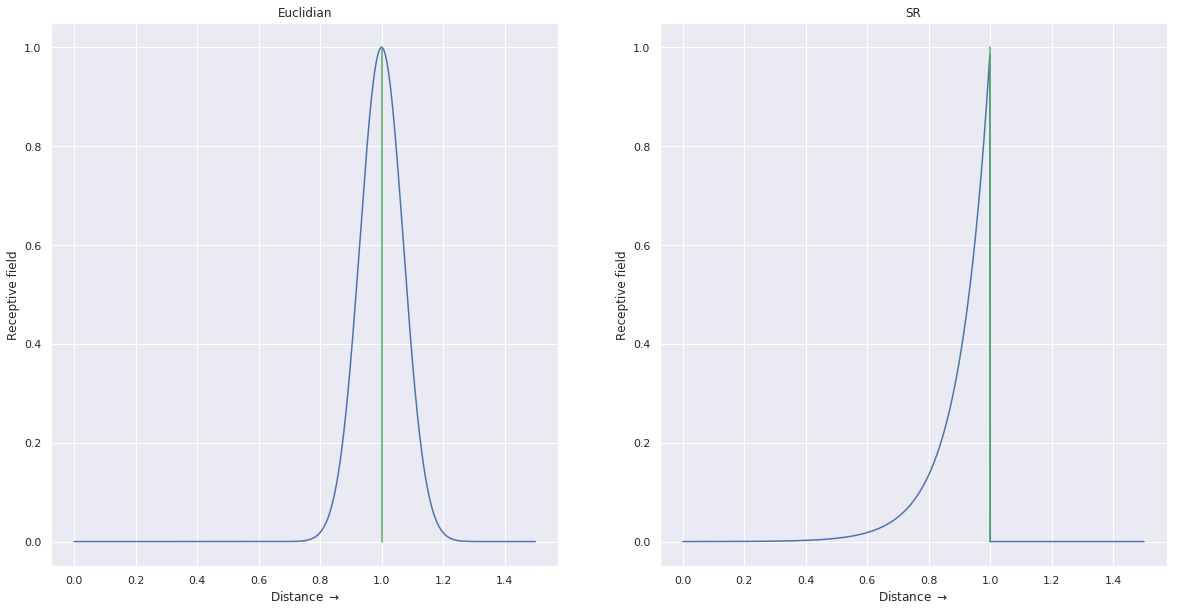
\includegraphics{img/sr_track.png}
\caption{\textbf{Figure 3.} Place field on a linear track with an
obstacle at x=1, using a Euclidian model (left) and the SR hypothesis
(right). Adapted from Fig. 2 of (Stachenfeld et al., 2017).}
\end{figure}

Fig. 3 illustrates this prediction: if a rat is placed on a linear track
with an obstacle, the place cell whose RF is centered on the obstacle
would react identically on both sides of the obstacle using a Euclidian
model, while it would only respond on the side it has explored using the
SR. When the rat is put on the other side, the SRs would initially be 0
for that cell (but would grow with more exploration).

Stachenfeld et al.~(2017) also propose a mechanism for grid cell
formation in the entorhinal cortex. Grid cells are understood as a
low-dimensional eigendecomposition of the SR place cells (dimensionality
reduction, as in principal component analysis). This allows to explain
why grid cells change in different environments (circular, rectangular
or triangular), as experimentally observed. They also propose a
mechanism for sub-goal formation using grid cells, but using the
normalized min-cut algorithm, so quite far from being biologically
realistic.

\hypertarget{discussion}{%
\section{Discussion}\label{discussion}}

Successor representations are an interesting trade-off between
model-free and model-based RL algorithms, explicitly separating state
transitions from reward estimation. It allows reacting quickly to distal
reward changes without the computational burden of completely
model-based planning. Deep RL variants of SR (Kulkarni et al., 2016)
obtain satisfying results on classical RL tasks such as Atari games and
simulated robots, but are still outperformed by modern model-free
algorithms. Similar to human behavior, hybrid architectures using both
SR and MF methods might be able to combine the optimality of MF methods
with the flexibility of the SR.

At the neuroscientific level, the SR hypothesis raises a lot of
interesting questions, especially regarding the interplay between the
prefrontal cortex, the hippocampus, and the basal ganglia during
goal-directed behavior. Here are just a few aspects that need to be
investigated both experimentally and theoretically:

\begin{itemize}
\tightlist
\item
  What is the relationship between the RPE and the SPE? Does VTA compute
  the SPE (still to be proven) and send it directly to the hippocampus
  through dopaminergic projections? Or does the RPE VTA somehow
  ``train'' ACC and PFC to compute the SPE, what is then sent to the
  hippocampus to update the SR representation? How?
\item
  How does the hippocampus learn from SPE signals? The SR hypothesis
  still has to be linked with evidence on plasticity in the hippocampus.
\item
  If dopamine does not carry the SPE, what is the role of the
  dopaminergic innervation of the hippocampus? The SR representation is
  in principle independent from rewards (except that animals may spend
  more time around reward location).
\item
  How is the value of a state / action computed based on the SR
  representation in the hippocampus? Do sharp wave ripples (SWR, also
  called forward/inverse replays) actually sample the SR matrix (a list
  of achievable states from the current one), what is then integrated
  elsewhere (ventral striatum?) to guide behavior?
\end{itemize}

\hypertarget{references}{%
\section*{References}\label{references}}
\addcontentsline{toc}{section}{References}

\hypertarget{refs}{}
\begin{CSLReferences}{1}{0}
\leavevmode\vadjust pre{\hypertarget{ref-Barreto2016}{}}%
Barreto, A., Dabney, W., Munos, R., Hunt, J. J., Schaul, T., van
Hasselt, H., et al. (2016). Successor {Features} for {Transfer} in
{Reinforcement Learning}. \emph{arXiv:1606.05312 {[}cs{]}}. Available
at: \url{http://arxiv.org/abs/1606.05312} {[}Accessed March 11, 2019{]}.

\leavevmode\vadjust pre{\hypertarget{ref-Corbit2011}{}}%
Corbit, L. H., and Balleine, B. W. (2011). The general and
outcome-specific forms of {Pavlovian}-instrumental transfer are
differentially mediated by the nucleus accumbens core and shell.
\emph{The Journal of neuroscience : the official journal of the Society
for Neuroscience} 31, 11786--94.
doi:\href{https://doi.org/10.1523/JNEUROSCI.2711-11.2011}{10.1523/JNEUROSCI.2711-11.2011}.

\leavevmode\vadjust pre{\hypertarget{ref-Dayan1993}{}}%
Dayan, P. (1993). Improving {Generalization} for {Temporal Difference
Learning}: The {Successor Representation}. \emph{Neural Computation} 5,
613--624.
doi:\href{https://doi.org/10.1162/neco.1993.5.4.613}{10.1162/neco.1993.5.4.613}.

\leavevmode\vadjust pre{\hypertarget{ref-Dickinson2002}{}}%
Dickinson, A., and Balleine, B. (2002). {``The role of learning in the
operation of motivational systems,''} in \emph{Steven's handbook of
experimental psychology: Learning, motivation, and emotion, {Vol}. 3,
3rd ed} ({Hoboken, NJ, US}: {John Wiley \& Sons Inc}), 497--533.

\leavevmode\vadjust pre{\hypertarget{ref-Doll2012}{}}%
Doll, B. B., Simon, D. A., and Daw, N. D. (2012). The ubiquity of
model-based reinforcement learning. \emph{Current Opinion in
Neurobiology} 22, 1075--1081.
doi:\href{https://doi.org/10.1016/j.conb.2012.08.003}{10.1016/j.conb.2012.08.003}.

\leavevmode\vadjust pre{\hypertarget{ref-Gardner2018}{}}%
Gardner, M. P. H., Schoenbaum, G., and Gershman, S. J. (2018).
Rethinking dopamine as generalized prediction error. \emph{Proceedings
of the Royal Society B: Biological Sciences} 285, 20181645.
doi:\href{https://doi.org/10.1098/rspb.2018.1645}{10.1098/rspb.2018.1645}.

\leavevmode\vadjust pre{\hypertarget{ref-Gershman2018}{}}%
Gershman, S. J. (2018). The {Successor Representation}: Its
{Computational Logic} and {Neural Substrates}. \emph{The Journal of
neuroscience : the official journal of the Society for Neuroscience} 38,
7193--7200.
doi:\href{https://doi.org/10.1523/JNEUROSCI.0151-18.2018}{10.1523/JNEUROSCI.0151-18.2018}.

\leavevmode\vadjust pre{\hypertarget{ref-Gershman2012}{}}%
Gershman, S. J., Moore, C. D., Todd, M. T., Norman, K. A., and
Sederberg, P. B. (2012). The {Successor Representation} and {Temporal
Context}. \emph{Neural Computation} 24, 1553--1568.
doi:\href{https://doi.org/10.1162/NECO_a_00282}{10.1162/NECO\_a\_00282}.

\leavevmode\vadjust pre{\hypertarget{ref-Kulkarni2016}{}}%
Kulkarni, T. D., Saeedi, A., Gautam, S., and Gershman, S. J. (2016).
Deep {Successor Reinforcement Learning}. \emph{arXiv:1606.02396 {[}cs,
stat{]}}. Available at: \url{http://arxiv.org/abs/1606.02396}
{[}Accessed February 20, 2019{]}.

\leavevmode\vadjust pre{\hypertarget{ref-Lee2014}{}}%
Lee, S. W., Shimojo, S., and O'Doherty, J. P. (2014). Neural
{Computations Underlying Arbitration} between {Model}-{Based} and
{Model}-free {Learning}. \emph{Neuron} 81, 687--699.
doi:\href{https://doi.org/10.1016/j.neuron.2013.11.028}{10.1016/j.neuron.2013.11.028}.

\leavevmode\vadjust pre{\hypertarget{ref-Ma2018}{}}%
Ma, C., Wen, J., and Bengio, Y. (2018). Universal {Successor
Representations} for {Transfer Reinforcement Learning}.
\emph{arXiv:1804.03758 {[}cs, stat{]}}. Available at:
\url{http://arxiv.org/abs/1804.03758} {[}Accessed February 23, 2019{]}.

\leavevmode\vadjust pre{\hypertarget{ref-Machado2018}{}}%
Machado, M. C., Bellemare, M. G., and Bowling, M. (2018). Count-{Based
Exploration} with the {Successor Representation}. \emph{arXiv:1807.11622
{[}cs, stat{]}}. Available at: \url{http://arxiv.org/abs/1807.11622}
{[}Accessed February 23, 2019{]}.

\leavevmode\vadjust pre{\hypertarget{ref-Miller2018}{}}%
Miller, K., Ludvig, E. A., Pezzulo, G., and Shenhav, A. (2018).
{``Re-aligning models of habitual and goal-directed decision-making,''}
in \emph{Goal-{Directed Decision Making} : Computations and {Neural
Circuits}}, eds. A. Bornstein, R. W. Morris, and A. Shenhav ({Academic
Press}). Available at:
\url{https://www.elsevier.com/books/goal-directed-decision-making/morris/978-0-12-812098-9}
{[}Accessed December 11, 2018{]}.

\leavevmode\vadjust pre{\hypertarget{ref-Momennejad2017a}{}}%
Momennejad, I., Russek, E. M., Cheong, J. H., Botvinick, M. M., Daw, N.
D., and Gershman, S. J. (2017). The successor representation in human
reinforcement learning. \emph{Nature Human Behaviour} 1, 680--692.
doi:\href{https://doi.org/10.1038/s41562-017-0180-8}{10.1038/s41562-017-0180-8}.

\leavevmode\vadjust pre{\hypertarget{ref-Stachenfeld2017}{}}%
Stachenfeld, K. L., Botvinick, M. M., and Gershman, S. J. (2017). The
hippocampus as a predictive map. \emph{Nature Neuroscience} 20,
1643--1653. doi:\href{https://doi.org/10.1038/nn.4650}{10.1038/nn.4650}.

\leavevmode\vadjust pre{\hypertarget{ref-Sutton2017}{}}%
Sutton, R. S., and Barto, A. G. (2017). \emph{Reinforcement {Learning}:
An {Introduction}}. Second. {Cambridge, MA}: {MIT Press} Available at:
\url{http://incompleteideas.net/book/the-book-2nd.html}.

\leavevmode\vadjust pre{\hypertarget{ref-Vitay2014}{}}%
Vitay, J., and Hamker, F. H. (2014). Timing and expectation of reward: A
neuro-computational model of the afferents to the ventral tegmental
area. \emph{Frontiers in Neurorobotics} 8.
doi:\href{https://doi.org/10.3389/fnbot.2014.00004}{10.3389/fnbot.2014.00004}.

\leavevmode\vadjust pre{\hypertarget{ref-Zhang2016}{}}%
Zhang, J., Springenberg, J. T., Boedecker, J., and Burgard, W. (2016).
Deep {Reinforcement Learning} with {Successor Features} for {Navigation}
across {Similar Environments}. \emph{arXiv:1612.05533 {[}cs{]}}.
Available at: \url{http://arxiv.org/abs/1612.05533} {[}Accessed March
11, 2019{]}.

\end{CSLReferences}

\end{document}
